\documentclass[aspectratio=169, 8pt]{beamer}
% \geometry{papersize={12.8cm,9.7cm}}

\usetheme[width=4\baselineskip]{Berkeley}
%% packages

%%%%%%%%%%%%%%%%%%%%%%%%%%%%%%%%%%%%%%%%%%%%%%%%%%%%%%%%%%%%%%%%%%%%%%%%%%%%%%
% \embedvideo{<poster or text>}{<video file (MP4+H264)>}
% \embedvideo*{...}{...}                     % auto-play
%%%%%%%%%%%%%%%%%%%%%%%%%%%%%%%%%%%%%%%%%%%%%%%%%%%%%%%%%%%%%%%%%%%%%%%%%%%%%%
\usepackage[bigfiles]{pdfbase}
\ExplSyntaxOn
\NewDocumentCommand\embedvideo{smm}{
  \group_begin:
  \leavevmode
  \tl_if_exist:cTF{file_\file_mdfive_hash:n{#3}}{
    \tl_set_eq:Nc\video{file_\file_mdfive_hash:n{#3}}
  }{
    \IfFileExists{#3}{}{\GenericError{}{File~`#3'~not~found}{}{}}
    \pbs_pdfobj:nnn{}{fstream}{{}{#3}}
    \pbs_pdfobj:nnn{}{dict}{
      /Type/Filespec/F~(#3)/UF~(#3)
      /EF~<</F~\pbs_pdflastobj:>>
    }
    \tl_set:Nx\video{\pbs_pdflastobj:}
    \tl_gset_eq:cN{file_\file_mdfive_hash:n{#3}}\video
  }
  %
  \pbs_pdfobj:nnn{}{dict}{
    /Type/RichMediaInstance/Subtype/Video
    /Asset~\video
    /Params~<</FlashVars (
      source=#3&
      skin=SkinOverAllNoFullNoCaption.swf&
      skinAutoHide=true&
      skinBackgroundColor=0x5F5F5F&
      skinBackgroundAlpha=0.75
    )>>
  }
  %
  \pbs_pdfobj:nnn{}{dict}{
    /Type/RichMediaConfiguration/Subtype/Video
    /Instances~[\pbs_pdflastobj:]
  }
  %
  \pbs_pdfobj:nnn{}{dict}{
    /Type/RichMediaContent
    /Assets~<<
      /Names~[(#3)~\video]
    >>
    /Configurations~[\pbs_pdflastobj:]
  }
  \tl_set:Nx\rmcontent{\pbs_pdflastobj:}
  %
  \pbs_pdfobj:nnn{}{dict}{
    /Activation~<<
      /Condition/\IfBooleanTF{#1}{PV}{XA}
      /Presentation~<</Style/Embedded>>
    >>
    /Deactivation~<</Condition/PI>>
  }
  %
  \hbox_set:Nn\l_tmpa_box{#2}
  \tl_set:Nx\l_box_wd_tl{\dim_use:N\box_wd:N\l_tmpa_box}
  \tl_set:Nx\l_box_ht_tl{\dim_use:N\box_ht:N\l_tmpa_box}
  \tl_set:Nx\l_box_dp_tl{\dim_use:N\box_dp:N\l_tmpa_box}
  \pbs_pdfxform:nnnnn{1}{1}{}{}{\l_tmpa_box}
  %
  \pbs_pdfannot:nnnn{\l_box_wd_tl}{\l_box_ht_tl}{\l_box_dp_tl}{
    /Subtype/RichMedia
    /BS~<</W~0/S/S>>
    /Contents~(embedded~video~file:#3)
    /NM~(rma:#3)
    /AP~<</N~\pbs_pdflastxform:>>
    /RichMediaSettings~\pbs_pdflastobj:
    /RichMediaContent~\rmcontent
  }
  \phantom{#2}
  \group_end:
}
\ExplSyntaxOff
%%%%%%%%%%%%%%%%%%%%%%%%%%%%%%%%%%%%%%%%%%%%%%%%%%%%%%%%%%%%%%%%%%%%%%%%%%%%%%
\usepackage{animate}
\usepackage{multimedia,graphicx,xcolor,transparent,textpos,relsize,tikz} %Addmultimidia
\usepackage{perpage} %the perpage package
\MakePerPage{footnote} 
% \usepackage{dtk-logos,tgpagella}
\usetikzlibrary{decorations.pathreplacing}
\newcommand{\tikzmark}[1]{\tikz[overlay,remember picture] \node[baseline] (#1) {};}
\tikzset{My Node Style/.style={midway, right, xshift=3.0ex, align=left, font=\small, draw=none, thin, text=black}}
\newcommand\VerticalBrace[4][]{%
    % #1 = draw options
    % #2 = top mark
    % #2 = bottom mark
    % #4 = label
\begin{tikzpicture}[overlay,remember picture]
  \draw[decorate,decoration={brace, amplitude=1.5ex}, #1] 
    ([yshift=1ex]#2.north east)  -- ([yshift=-1ex]#3.south east)
        node[My Node Style] {#4};
\end{tikzpicture}
}


\definecolor{codegreen}{rgb}{0,0.6,0}
\definecolor{codegray}{rgb}{0.5,0.5,0.5}
\definecolor{codepurple}{rgb}{0.58,0,0.82}
\definecolor{backcolour}{rgb}{0.95,0.95,0.92}
\definecolor{lightgrey}{rgb}{0.9,0.9,0.9}
\definecolor{darkgreen}{rgb}{0,0.6,0}
\definecolor{folderbg}{RGB}{124,166,198}
\definecolor{folderborder}{RGB}{110,144,169}

\usepackage{listings,lstautogobble}
\usepackage[edges]{forest}

\usepackage{graphicx,xcolor,transparent,textpos} %Addmultimidia

\newcommand\hmmax{0}
\newcommand\bmmax{0}

\usepackage{amsmath, amssymb, amsfonts, amsthm, bm}

\usepackage[none]{hyphenat}

\usepackage{booktabs, multirow} %for tables

\usepackage{siunitx}

\usepackage[brazil]{babel}

\usepackage{caption, threeparttable} \captionsetup{font=footnotesize,skip=0.06pt}
\captionsetup[figure]{labelformat=empty}

\usepackage[doi=false, isbn=false, doi=false, style=numeric, sorting=none]{biblatex}

\usepackage{times, helvet, ebgaramond, lmodern}
\newcommand*{\tim}{\fontfamily{ptm}\selectfont}
\newcommand*{\helv}{\fontfamily{phv}\selectfont}
\newcommand*{\gara}{\fontfamily{EBGaramond-LF}\selectfont}
\newcommand*{\cmu}{\fontfamily{cmr}\selectfont}

\usepackage{palatino}
%citation options%
\AtEveryCitekey{%
\ifentrytype{article}
    {\clearfield{url}\clearfield{urlyear}}
    {}%
}
\usetheme{Berkeley} % theme for slides
\usefonttheme{serif} 
\definecolor{c1}{RGB}{255,255,0} % some yellow
\definecolor{c2}{RGB}{1,33,105} % some blue
\setbeamercolor{palette primary}{fg=white, bg=c2} % upper part
\setbeamercolor{palette secondary}{fg=white, bg=c2} % left part (background)
\setbeamercolor{sidebar left}{fg=white, bg=c2} % left part with links
\setbeamercolor{section number projected}{bg=c2} % color of section numbers and others 
\setbeamercolor{item projected}{bg=c2}
\setbeamercolor{itemize item}{fg=c2}
\setbeamercolor{author in sidebar}{fg=white}
\setlength\parindent{0pt}

\logo{
\includegraphics[width=1.3cm,height=1.3cm,keepaspectratio]{build/logo}}

%%%%%%%Logo lower left
\addtobeamertemplate{headline}{}{
\begin{textblock*}{100mm}(2mm, 6.6cm)
\includegraphics[height=1.2cm,width=1.2cm,keepaspectratio]{build/usp} % logo of my university
\end{textblock*}}

%%%%%%%Logo upper mid
%\addtobeamertemplate{headline}{}{
%\begin{textblock*}{100mm}(12cm, -1.32cm)
%\includegraphics[height=1.5cm,width=1.5cm,keepaspectratio]{figures/lfslogo} % logo of my university
%\end{textblock*}}

%%%%%%%Logo upper right
\addtobeamertemplate{headline}{}{
\begin{textblock*}{100mm}(13cm, -1.0cm)

\includegraphics[height=1.8cm,width=1.8cm,keepaspectratio]{build/pmtpolilogo} % logo of my university
\end{textblock*}}

% \usefonttheme{professionalfonts} % changes fonts
% \setbeamerfont{normal text}{size*={9}}

\setbeamerfont{section number projected}{ % section numbers
  family=\rmfamily,
  series=\bfseries,
  size=\footnotesize
  }

% \usenavigationsymbolstemplate{}% deafult controls off 
% \setbeamertemplate{footline}[frame number] % slide number at the bottom

\newcommand{\cm}[1]{{\tt \textcolor{orange}{#1}}}
\newcommand{\wl}[2]{\href{#2}{\textcolor{blue}{#1}}}
\newcommand{\att}[2]{\href{#2}{\textcolor{blue}{#1}}}
\definecolor{codegreen}{rgb}{0,0.6,0}
\definecolor{codegray}{rgb}{0.5,0.5,0.5}
\definecolor{codepurple}{rgb}{0.58,0,0.82}
\definecolor{backcolour}{rgb}{0.95,0.95,0.92}
%toprule width TABELA TOP LINHA
\newlength{\toprulewidth}
\setlength{\toprulewidth}{0.25ex}
\patchcmd{\toprule}% <cmd>
  {\heavyrulewidth}{\toprulewidth}% <search><replace>
  {}{}% <success><failure>
  
 %bottom rule width TABELA BOT LINHA
  \newlength{\bottomrulewidth}
\setlength{\bottomrulewidth}{0.25ex}
\patchcmd{\bottomrule}% <cmd>
  {\heavyrulewidth}{\bottomrulewidth}% <search><replace>
  {}{}% <success><failure>

\setbeamertemplate{footline}[frame number]{}

%# FOLDER TREES PACKAGE MACRO
\usepackage{array}
\definecolor{folderbg}{RGB}{124,166,198}
\definecolor{folderborder}{RGB}{110,144,169}
\newlength\Size
\setlength\Size{4pt}
\tikzset{%
  folder/.pic={%
    \filldraw [draw=folderborder, top color=folderbg!50, bottom color=folderbg] (-1.05*\Size,0.2\Size+5pt) rectangle ++(.75*\Size,-0.2\Size-5pt);
    \filldraw [draw=folderborder, top color=folderbg!50, bottom color=folderbg] (-1.15*\Size,-\Size) rectangle (1.15*\Size,\Size);
  },
  file/.pic={%
    \filldraw [draw=folderborder, top color=folderbg!5, bottom color=folderbg!10] (-\Size,.4*\Size+5pt) coordinate (a) |- (\Size,-1.2*\Size) coordinate (b) -- ++(0,1.6*\Size) coordinate (c) -- ++(-5pt,5pt) coordinate (d) -- cycle (d) |- (c) ;
  },
}
\forestset{%
  declare autowrapped toks={pic me}{},
  declare boolean register={pic root},
  pic root=0,
  pic dir tree/.style={%
    for tree={%
      folder,
      font=\itshape,
      grow'=0,
    },
    before typesetting nodes={%
      for tree={%
        edge label+/.option={pic me},
      },
      if pic root={
        tikz+={
          \pic at ([xshift=\Size].west) {folder};
        },
        align={l}
      }{},
    },
  },
  pic me set/.code n args=2{%
    \forestset{%
      #1/.style={%
        inner xsep=2\Size,
        pic me={pic {#2}},
      }
    }
  },
  pic me set={directory}{folder},
  pic me set={file}{file},
}
\newcommand{\fname}[2]{\begin{tabular}{m{1cm}@{\quad}m{4cm}}#1 & \normalfont#2\end{tabular}}

\addbibresource{Mini-curso_LaTeX.bib}
\fontfamily{cmr}\selectfont
\makeatletter
\beamer@headheight=4.5\baselineskip
\makeatother

\begin{document}
\lstset{
	language={[LaTeX]TeX},
	xleftmargin=0em,
	xrightmargin=\dimexpr\fboxsep+\fboxrule,
	breaklines=true,
	keywordstyle=\color{blue}\sf,
	% identifierstyle=\color{magenta},
	commentstyle=\scriptsize\color{cyan},
	tabsize=2,
	morekeywords={text},
	columns=flexible,
	backgroundcolor=\color{backcolour},
	stringstyle=\color{black},
	basicstyle=\ttfamily\footnotesize,
	breakatwhitespace=false,
	captionpos=b,
	keepspaces=true,
	numbers=left,
	numbersep=5pt,
	showspaces=false,
	showstringspaces=false,
	showtabs=false,
	autogobble=true,        
	literate={ã}{{\~a}}1
	{ç}{{\c{c}}}1
	{é}{{\'e}}1
	{ú}{{\'u}}1
	{ê}{{\^e}}1
	{á}{{\'a}}1
	{ó}{{\'o}}1
}          
% Set your language (you can change the language for each code-block optionally)

%info
\title[mini-curso de \LaTeX]{mini-curso de \LaTeX}
\author[\sc Juan Manuel]{Juan Manuel Costa Miscione}
\date[2022]{\small 2022}


\begin{frame}
	\titlepage
	\vfill
	\usebeamerfont{institute} contato: \url{omanuelcosta@protonmail.com}
\end{frame}

\section{Introdução}
\begin{frame}{Introdução}
	\tableofcontents
\end{frame}
	\begin{frame}{Introdução}
		\tableofcontents[currentsection, hidesubsections]
	\end{frame}

	\begin{frame}{O que é o \LaTeX\ e como ele funciona?}
		\pause
		\LaTeX\ é uma ferramenta para produção de documentos.
		\pause
		\begin{figure}
			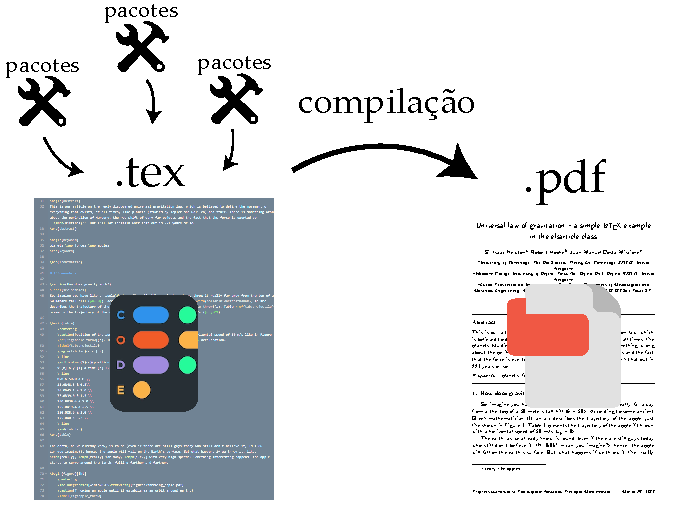
\includegraphics[width=0.5\textwidth]{figures/LaTeX_basics.pdf}
		\end{figure}

	\end{frame}

	\begin{frame}{Porque e quando usar o \LaTeX ?}
		\pause
		{\Large\center{\LaTeX}}
		\vspace{1em}
		
		\begin{tabular*}{\textwidth}[c]{c @{\extracolsep{\fill}} c c}
			Pros: & Cons: &
		\end{tabular*}\vspace{0.5em}
		\pause
		\begin{minipage}{0.5\textwidth}
			\begin{itemize}
				\item melhor formatação e qualidade tipográfica
				\item menos tempo gasto em formatação
				\item melhor notação matemática
				\item melhor gerenciamento bibliográfico
			\end{itemize}
		\end{minipage}%
		\pause
		\begin{minipage}{0.5\textwidth}
			\begin{itemize}
				\item curva rasa de aprendizado
				\item requer a utilização de um gerenciador de pacotes\footnote{resolvido pelo Overleaf.}
				\item soluções para problemas devem ser procurados online$^\text{\emph{a}}$
			\end{itemize}
		\end{minipage}
		\pause
		{\Large\center{MS Word}}
		\vspace{1em}
		
		\begin{tabular*}{\textwidth}[c]{c @{\extracolsep{\fill}} c c}
			Pros: & Cons: &
		\end{tabular*}\vspace{0.5em}
		\pause
		\begin{minipage}{0.5\textwidth}
			\begin{itemize}
				\item boa curva de aprendizado (WYSWYG)
				\item disponibilidade
			\end{itemize}
		\end{minipage}%
		\pause
		\begin{minipage}{0.5\textwidth}
			\begin{itemize}
				\item baixa qualidade tipográfica
				\item desconfiguração (explosões)
				\item mau versionamento
			\end{itemize}
		\end{minipage}
	\end{frame}
	
	\begin{frame}{MS Word vs \LaTeX}
		\center{
			\includegraphics[width=0.66\textwidth]{figures/latex_vs_word_gráfico.pdf}
		}
	\end{frame}
	\begin{frame}{MS Word vs \LaTeX}
		\center{
			
\includegraphics[width=0.65\textwidth]{figures/latex meme.jpg}
		}
	\end{frame}
	\begin{frame}{MS Word vs \LaTeX}
		\center{
			
\includegraphics[width=0.46\textwidth]{figures/latex_fan.pdf}
		}
	\end{frame}

	\begin{frame}{O que é WYSWYG? (\emph{what you see what you get})}
		\begin{figure}
			\centering
			
\includegraphics[width=\textwidth]{figures/WYSWYG.pdf}
		\end{figure}

		\pause

		Em programas modernos, do tipo ``WYSWYG'' (trad. \emph{o que você vê é o que você tem}), a edição direta no documento é interpretado pelo software.

		\vspace{1em}

		Com o \LaTeX, a edição é diretamente em cima do código. Isso evita ``\emph{explosões}'' em documentos grandes e com alta complexidade (referências, citações, legendas).

	\end{frame}

\section{Estrutura e formatação}
\begin{frame}{Estrutura, formatação e exemplos}
	\tableofcontents[currentsection, hidesubsections]
\end{frame}

	\begin{frame}{uma figura e uma legenda}
		\begin{columns}
			\column{0.5\textwidth}
				\begin{figure}
					\centering
					\animategraphics[width=\textwidth]{8}{figures/examplesvideo/}{1}{95}
				\end{figure}
			\column{0.5\textwidth}
				\begin{figure}
					\centering	
					\animategraphics[width=\textwidth]{5}{figures/examplewordvideo/}{1}{50}
				\end{figure}
		\end{columns}
	\end{frame}

	\begin{frame}[fragile]{comandos (\textbackslash), opções [\emph{opt}], argumentos \{ \emph{args} \}}
		
		\pause

		comandos, em \LaTeX, são iniciados por \textbackslash :
		\begin{itemize}
			\item \textbf{\textbackslash \emph{documentclass}}[opt]\{ args \}
			\item \textbf{\textbackslash \emph{usepackage}}[opt]\{ args \}
			\item \textbf{\textbackslash \emph{begin}} \{ args \}
		\end{itemize}
		\pause

		as opções são incluídas entre [ ]:
		\begin{itemize}
			\item \textbackslash \emph{documentclass}[\textbf{11pt}, \textbf{a4paper}, \textbf{twocolumns}]\{ args \}
			\item \textbackslash \emph{usepackage}[\textbf{style=numeric}, \textbf{sorting=none}]\{ biblatex \}
			\item \textbackslash \emph{includegraphics} [\textbf{width=\emph{n}}, \textbf{angle=\emph{n}}] \{ args \}
		\end{itemize}

		\pause
		os argumentos são colocados dentro de \{ \}:
		\begin{itemize}
			\item \textbackslash \emph{documentclass}[opt]\{ \textbf{article},\textbf{report}, \emph{etc} \}
			\item \textbackslash \emph{usepackage}[opt]\{ \textbf{amsmath}, \textbf{biblatex}, \textbf{hyperref}, \emph{etc} \}
			\item \textbackslash \emph{begin} \{ \textbf{document}, \textbf{figure}, \textbf{table}, \emph{etc} \}
		\end{itemize}



	\end{frame}

	\begin{frame}[fragile]{Estrutura do documento\footnote{Para mais informações sobre a estrutura de documentos \LaTeX\ -- \textcite{LaTeXDocumentStructure}}}
		\begin{columns}
			\column{0.5\textwidth}
			\centering
				\begin{lstlisting}
					\documentclass[options]{class}
					\usepackage{a,b,c,d...}

					\begin{document}
						Hello Word
					\end{document}
				\end{lstlisting}
			\column{0.5\textwidth}
				\begin{figure}
					\fbox{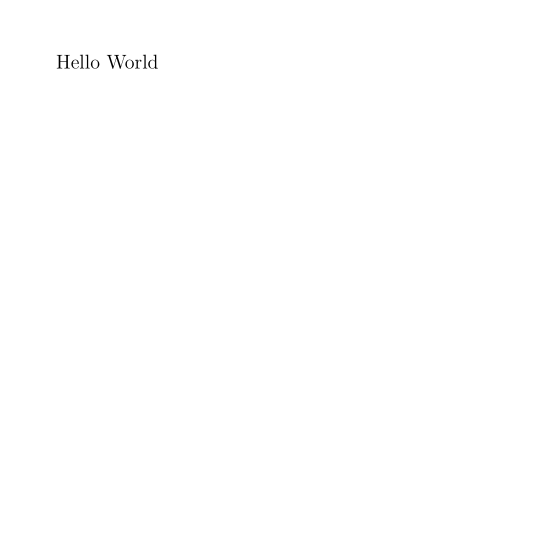
\includegraphics[width=0.7\textwidth]{figures/helloworld.PNG}}
				\end{figure}
			\end{columns}

			\pause

			\begin{itemize}
				\centering
				\item \emph{options} = fonte (10pt, 11pt), papel (a4paper, letterpaper), draft, colunas.
				\item \emph{class} = article, proc, report, book, memoir, beamer (atual).
				\item \emph{usepackage} = amsmath, amssymb, hyperref, bibla\TeX, babel
			\end{itemize}
	\end{frame}

	\begin{frame}[fragile]{Imagem e legenda - environments e floats}

		\begin{columns}
			\column{0.48\textwidth}
				iniciamos o comando \textbackslash includegraphics[]\{\} disponibilizado pelo pacote \emph{graphicx}, 

				ajustamos a largura nas opções entre [] e o caminho da figura entre \{\}
				\begin{lstlisting}
					\documentclass[11pt]{article}
					\usepackage{graphicx}

					\begin{document}

						\begin{figure}
							\centering 
							\includegraphics[width=0.85\textwidth]
							{example_figure.pdf} 
							\caption{Uma figura em \LaTeX}
						\end{figure}
						
					\end{document}
				\end{lstlisting}
			\column{0.3\textwidth}
				\fbox{
\includegraphics[width=\textwidth]{examples/figure_example/example-figure.pdf}}
		\end{columns}
	\end{frame}

	\begin{frame}[fragile]{o que é \textbackslash\emph{textwidth}\footnote{\textcite{LaTeXLengthsWikibooks}}}
		
		\pause
		{\centering O \textbackslash textwidth refere-se a medida horizontal do total disponível para texto na folha (página A4 - margens). Outras medidas:}

		\vspace{1em}
		
		\begin{itemize}
			\item[] \textbackslash\emph{baselineskip} -- a distância horizontal entre duas linhas
			\item[] \textbackslash\emph{paperwidth} -- largura da página
			\item[] \textbackslash\emph{textheight} -- altura da região do texto na página
		\end{itemize}

		\vspace{1em}

		\textbackslash includegraphics[width=\emph{n}\textbackslash textwidth]\{figure.jpg/png/pdf\},
		Onde \emph{n} é um multiplicador (1.0, 0.8, 0.5).
		
	\end{frame}

	\begin{frame}{o que é \textbackslash\emph{textwidth}}
		\begin{figure}
			\centering
			\fbox{\animategraphics[autoplay, loop, width=0.35\textwidth]{0.7}{examples/figure_width/gif/}{1}{3}}
		\end{figure}
	\end{frame}
	
	\begin{frame}[fragile]{Notação matemática\footnote{\textcite{LaTeXMathematicsWikibooks}}}

		\begin{center}
			Como escrever equações matemáticas?
		\end{center}

		\pause

		O modo matemático é ativado colocando a equação entre \textcolor{red}{\$} x\^{}2 \textcolor{red}{\$} (modo \emph{inline}), \textcolor{red}{\textbackslash [} x\^{}2 \textcolor{red}{\textbackslash ]} ou \textcolor{red}{\textbackslash begin\{equation\}} x\^{}2 \textcolor{red}{\textbackslash end\{equation\}}, ou até mesmo \textcolor{red}{\textbackslash begin\{align\}}x\^{}2 \textcolor{red}{\textbackslash end\{align\}}\footnote{várias equações alinhadas | disponibilizado pelo pacote \textbf{amsmath}}

		\pause

		\begin{columns}
			\column{0.5\textwidth}
				\begin{lstlisting}{language=TeX}
					E = mc^2
				\end{lstlisting}

				\begin{lstlisting}{language=TeX}
					\text{d} S \geq 0
				\end{lstlisting}

				\begin{lstlisting}{language=TeX}
					F = G \frac{m_1 m_2}{r^2}
				\end{lstlisting}
			\column{0.5\textwidth}
					$E = mc^2$\\
					\vspace{1em}
					$\text{d}S \geq 0$\\
					\vspace{1em}
					$F = G \frac{m_1 m_2}{r^2}$\\
		\end{columns}
	\end{frame}
	
	\begin{frame}[fragile]{Notação matemática}
		\begin{columns}
			\column{0.5\textwidth}
				\begin{lstlisting}
					\documentclass[12pt,oneside,a4paper]{article}
					
					\begin{document}
						A famosa equação de Einstein, $E=m c^2$, 
						na sua forma completa é:
						\begin{equation}
							E^2 = (m c^2)^2 + (p c)^2
						\end{equation}
					\end{document}
				\end{lstlisting}
			\column{0.5\textwidth}
				\fbox{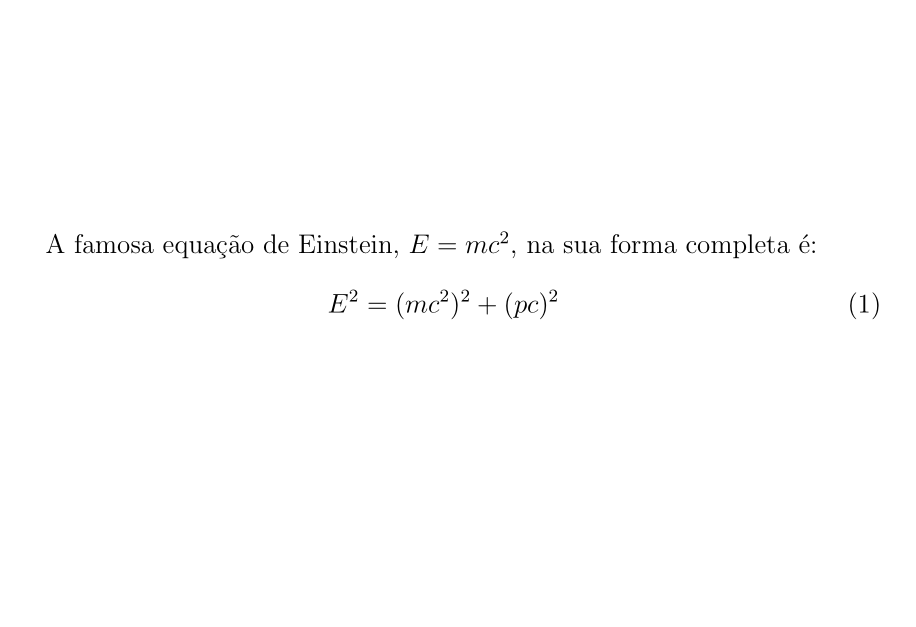
\includegraphics[width=0.65\textwidth]{examples/math/mathexample.PNG}}
		\end{columns}

		\pause

		\begin{columns}
			\column{0.5\textwidth}
				sub/superscrito, $x^2, x_0, a_{i+2}, {\alpha_0^2}^2_0$ \\
				\vspace{1em}
				raíz, $\sqrt{1-x^2}$ \\
				\vspace{1em}
				fração, $\frac{2\alpha^i}{\beta^n}$ \\
				\vspace{1em}
				integral, $\int_0^i f(x)\text{d}x$ \\
				\vspace{1em}
				símbolos, $\aleph_0$, $\uparrow$, $\prod$, $\in$, $\overbrace{abc}$ 

			\column{0.5\textwidth}
				\begin{lstlisting}
					x^2, x_0, a_{i+2}, {\alpha_0^2}^2_0
				\end{lstlisting}

				\begin{lstlisting}
					\sqrt{1-x^2}
				\end{lstlisting}

				\begin{lstlisting}
					\frac{2\alpha^i}{\beta^n}
				\end{lstlisting}

				\begin{lstlisting}
					\int_0^i f(x)dx
				\end{lstlisting}

				\begin{lstlisting}
					$\aleph_0$, $\uparrow$, $\prod$, 
					$\in$, $\overbrace{abc}$ 
				\end{lstlisting}
		\end{columns}
	\end{frame}

	\begin{frame}[fragile]{Formatação\footnote{\textcite{LaTeXFontsWikibooks}}}

		{\centering
		Fonte $\neq$ Typeface

		\pause
		\vspace{1em}

		{\tim Times} é uma typeface, {\helv Helvetica} é uma typeface, {\gara Garamond} é uma typeface.\\
		\vspace{1em}
		\cmu{\textbf{Computer Modern em negrito}} é uma fonte, \cmu{\textit{Computer Modern em itálico}} é outra fonte.
		}

		\pause

		\begin{columns}
			\column{0.5\textwidth}
				\vspace{2em}
				\begin{lstlisting}
					\emph{ênfase}

					\textbf{negrito}

					\textsc{Small Caps}

					\tiny{muito pequeno}

					\small{pequeno}

					\Large{grande}

					% comentários são escritos
					% após o % (são ignorados na compilação)
				\end{lstlisting}
			\column{0.48\textwidth}
				\emph{ênfase} \\
				\vspace{0.7em}
				\textbf{negrito} \\
				\vspace{0.7em}
				\textsc{Small Caps} \\
				\vspace{0.7em}
				\tiny{muito pequeno} \\
				\vspace{0.7em}
				\small{pequeno} \\
				\vspace{0.7em}
				\Large{grande}

		\end{columns}
	\end{frame}

	\begin{frame}[fragile]{Tabelas\footnote{\textcite{LaTeXTablesWikibooks}}}

		\pause

		\begin{itemize}
			\item Utilizamos 2 ambientes para construir tabelas: o \textbackslash begin\{table\} e \textbackslash begin\{tabular\} \vspace{1em}
			\item O ambiente tabular é definido pelas colunas e seu alinhamento (c$\rightarrow$centro, l$\rightarrow$esquerda, r$\rightarrow$direita)
			\item As células são separadas em \& e as linhas em \textbackslash\textbackslash.
		\end{itemize}

		\pause

		\begin{columns}
			\column{0.48\textwidth}
				\begin{lstlisting}
					\begin{table}
						\begin{tabular}{l c c r}
							\hline
							amostra & $\delta_{ij}$ & $\alpha_{ij}$
							 & tempo (s) \\
							\hline
							1 & 23.1 & 32.4 & 16 \\
							2 & 42.1 & 65.4 & 17 \\
							3 & 55.1 & 82.4 & 23 \\
							\hline
						\end{tabular}
						\caption{um exemplo de Tabela no \LaTeX}
					\end{table}
				\end{lstlisting}
			\column{0.48\textwidth}
			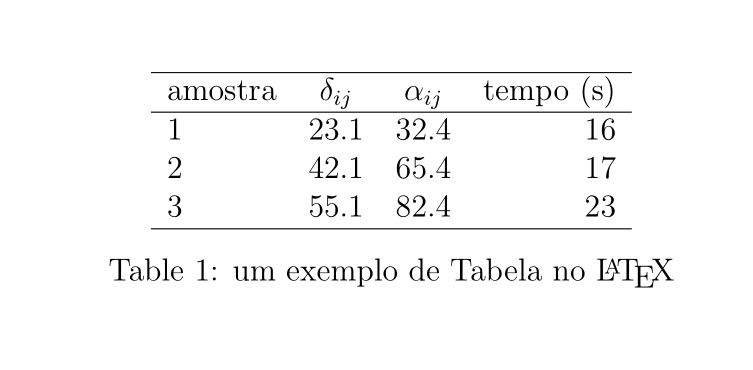
\includegraphics[width=\textwidth]{examples/tabelas/tabela_result.PNG}
		\end{columns}
	\end{frame}

\section{Labels, refs e notas}
\begin{frame}{}
	\tableofcontents[currentsection, hidesubsections]
\end{frame}

	\begin{frame}[fragile]{Labels}
		\begin{columns}
			\column{0.45\textwidth}
				\begin{lstlisting}
					\begin{figure}
						\centering
						
\includegraphics[width=0.6\textwidth]
						{meme_superior.png}
						\caption{Uma figura \LaTeX}
						\label{fig:meme}
					\end{figure}

					A Figura \ref{fig:meme} está na página 
					\pageref{fig:meme}.
				\end{lstlisting}
			\column{0.5\textwidth}
				
\includegraphics[width=0.7\textwidth]{examples/labels e refs/labels0.PNG}
		\end{columns}
	\end{frame}

	\begin{frame}[fragile]{Labels e cross-references\footnote{\textcite{LaTeXLabelsWikibooks}}}

		{
			\centering\small
			O \textbackslash label no \LaTeX\ serve para referenciar uma Figura/Tabela/Equação no texto.

		}

		\begin{columns}
			\column{0.45\textwidth}
				\begin{lstlisting}[basicstyle=\tiny]
					\begin{figure}
						\includegraphics{figura1.png}
						\caption{Uma figura \LaTeX}
						\label{fig:meme}
					\end{figure}
					\begin{equation}
						E = m c ^2
					\end{equation}
					\begin{equation}\label{eqn:einsteincompleta}
						E^2 = (m c^2)^2 + (p c)^2
					\end{equation}
					\begin{table}
						\begin{tabular}{l c c r}
							\hline
							amostra & $\delta_{ij}$ & $\alpha_{ij}$
								& tempo (s) \\
							\hline
							1 & 23.1 & 32.4 & 16 \\
							2 & 42.1 & 65.4 & 17 \\
							3 & 55.1 & 82.4 & 23 \\
							\hline
						\end{tabular}
						\caption{Uma tabela \LaTeX}\label{tab:alpha_delta}
					\end{table}
					A Figura \ref{fig:meme} está na página 
					\pageref{fig:meme}. Já a Equação 
					\ref{eqn:einsteincompleta} foi usada 
					para produzir a Tabela \ref{tab:alpha_delta}
					que está na página \pageref{tab:alpha_delta}.
				\end{lstlisting}
			\column{0.5\textwidth}
				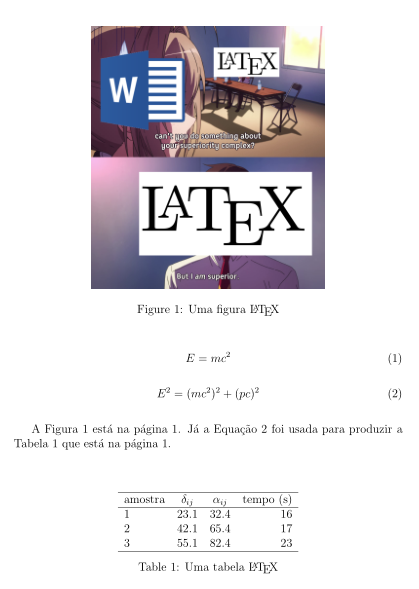
\includegraphics[width=0.7\textwidth]{examples/labels e refs/labels.png}
		\end{columns}
	\end{frame}


\section{Bibliografias}
	\begin{frame}[fragile]{Gerenciamento bibliográfico\footnote{\textcite{LaTeXBibliographyWikibooks}}}
		\pause
		Como adicionar uma lista de \emph{referências} e fazer \emph{citações}?

		\pause
		\vspace{2em}
		podemos escolher entre 3 ferramentas:
		\begin{itemize}
			\item bib\TeX
			\item natbib
			\item \textbf{Bibla\TeX}\footnote{versão mais ``\emph{moderna}'' e moderna, mas menos \emph{user-friendly}}
		\end{itemize}

	\end{frame}
	
	\begin{frame}[fragile]{Gerenciamento bibliográfico -- Bibla\TeX}

				\begin{itemize}
					\item Chamamos o pacote Bibla\TeX $\rightarrow$ \lstinline|\usepackage{biblatex}|
					\item Incluímos uma bibliografia \emph{.bib} no nosso documento $\rightarrow$ \lstinline|\addbibresource{nome_do_arquivo.bib}|
					\item Fazemos uma citação  $\rightarrow$ \lstinline{\cite}, \lstinline{\footcite}, \lstinline{\textcite}, \emph{et caetera}.
					\item Imprimimos as referências bibliográficas $\rightarrow$ \lstinline{\printbibliography}
				\end{itemize}

		\pause
		\vspace{2em}
			\begin{forest}
				pic dir tree,
				pic root,
				for tree={% folder icons by default; override using file for file icons
				  directory,
				},
				[pasta
				    [\fname{main.tex}{\hspace{3em}\fbox{arquivo \emph{.tex} contendo \textbackslash\emph{addbibresource} e \textbackslash\emph{cite}}}, file
				    ]
				    [\fname{referencias.bib}{\hspace{3em}\fbox{arquivo \emph{.bib} contendo as referências}}, file
				    ]
				]
			\end{forest}
	\end{frame}

	\begin{frame}[fragile]{O que há num arquivo \emph{.bib}?}

		\pause
		O arquivo \emph{.bib} contém referências (\emph{entries}) num formato específico produzido pelos principais gerenciadores bibliográficos -- \emph{Mendeley}, \emph{Zotero}, \emph{EndNote}, \emph{et caetera}.

		\pause
		\begin{columns}
			\column{0.7\textwidth}
				{\centering referências.bib}
				\begin{lstlisting}
					@book{heath2002works,
					title={The works of Archimedes},
					author={Heath, Thomas Little and others},
					year={2002},
					publisher={Courier Corporation}
					}

					@article{arnould2007r,
					title={The r-process of stellar nucleosynthesis: 
					Astrophysics and nuclear physics achievements and mysteries},
					author={Arnould, Marcel and Goriely, 
					St{\'e}phane and Takahashi, Kohji},
					journal={Physics Reports},
					volume={450},
					pages={97--213},
					year={2007},
					publisher={Elsevier}
					}
				\end{lstlisting}

			\column{0.28\textwidth}
			tipos de \emph{entry} ou entradas:
			\begin{itemize}
				\item @ book
				\item @ conference
				\item @ periodical
				\item @ collection
				\item @ report
			\end{itemize}
		\end{columns}
	\end{frame}

	\begin{frame}[fragile]{Gerenciamento bibliográfico -- Bibla\TeX}
		\begin{columns}
			\column{0.48\textwidth}
				\begin{tabular}{l}
					main.\emph{tex}\\
					\begin{lstlisting}
						\documentclass[12pt]{article}
						\usepackage{biblatex}
						\addbibresource{referencias.bib}

						\begin{document}
						Segundo Arquimedes \cite{heath2002works}, a area de 
						um circulo e $\pi r^2$

						\printbibliography
						\end{document}
					\end{lstlisting} \\[2.5em]
					referencias.\emph{bib} \\
					\begin{lstlisting}
						@book{heath2002works,
						title={The works of Archimedes},
						author={Heath, Thomas Little and others},
						year={2002},
						publisher={Courier Corporation}
						}
					\end{lstlisting}
				\end{tabular}
			\column{0.48\textwidth}
				\begin{figure}
					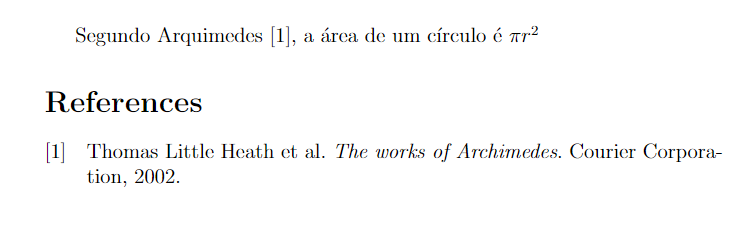
\includegraphics[width=\textwidth]{examples/bibliography/output.PNG}
				\end{figure}
		\end{columns}
	\end{frame}

	\begin{frame}{Como instalar o \LaTeX\ no meu computador?}

		\pause
		Para instalar o \LaTeX, você precisa de:
		\vspace{2em}
		\pause
		\begin{itemize}
			\item Uma distribuição \LaTeX\ (que gerencia os pacotes): \begin{itemize}
				\item \textbf{Mik\TeX}\footnote{\emph{user-friendly}}\cite{miktex}
				\item \TeX\ Live\cite{texlive}
				\item pro\TeX t\cite{protex}
					\end{itemize}
			\pause
			\vspace{2em}
			\item Um IDE (basicamente um editor de texto para códigos):
			\begin{itemize}
				\item \TeX\ Studio
				\item \textbf{\TeX\ Maker}$^1$\cite{texmaker}
				\item VSCode
			\end{itemize}

		\end{itemize}
		\pause
		\vspace{2em}
		Ou você pode começar imediatamente no Overleaf\cite{overleaf}.

	\end{frame}

	\begin{frame}{Modelos}
		Modelos disponíveis no Overleaf:
		\begin{itemize}
			\item \href{https://www.overleaf.com/latex/templates/modelo-canonico-de-trabalhos-academicos-com-abntex2/ybtpkzkccnnj}{\textcolor{blue}{Modelo Canônico de Trabalhos Acadêmicos com abn\TeX 2}}
			\item \href{https://www.overleaf.com/latex/templates?q=abntex2}{\textcolor{blue}{Galeria de modelos acadêmicos utilizando o abn\TeX 2}}
		\end{itemize}
		\vspace{1.5em}
		Materiais disponíveis neste minicurso:
		\begin{itemize}
			\item blabla
		\end{itemize}
		
	\end{frame}
%%%%%%%%%%%%%%%%%%%%%%%%%%%%%%%%%%%%%%%%%%%%%%%%%%%%%
\begin{frame}[allowframebreaks]{Referências}
\printbibliography
\end{frame}

\end{document}

%%%%%%%%%%%%%%%%%%%%%%%%%%%%%%%%%%%%%%%%%%%%%%%%%%%%%